\documentclass[a4paper,11pt]{article}

% Kodovani (cestiny) v dokumentu: utf-8
%\usepackage[cp1250]{inputenc}	% Omezena stredoevropska kodova stranka, pouze MSW.
\usepackage[utf8]{inputenc}	% Doporucujeme pouzivat UTF-8 (unicode).

\usepackage[margin=2cm]{geometry}
\newtoks\jmenopraktika \newtoks\jmeno \newtoks\datum
\newtoks\obor \newtoks\skupina \newtoks\rocnik \newtoks\semestr
\newtoks\cisloulohy \newtoks\jmenoulohy
\newtoks\tlak \newtoks\teplota \newtoks\vlhkost

\jmenopraktika={Fyzikální praktikum 1}
\jmeno={Lukáš Lejdar}
\datum={12. března 2024}
\obor={F}
\skupina={Út 16:00}

\cisloulohy={7}
\jmenoulohy={Měření Poissonovy konstanty vzduchu}

\tlak={98.4970}
\teplota={21,1}
\vlhkost={47.4}

%%%%%%%%%%% Uzitecne balicky:
\usepackage[czech]{babel}
\addto\captionsczech{\renewcommand{\figurename}{Graf}}

\usepackage{graphicx}
\usepackage{amsmath}
\usepackage{xspace}
\usepackage{url}
\usepackage{indentfirst}
\usepackage{wrapfig}
\usepackage{xcolor}
\usepackage{caption}

%%%%%% Zamezeni parchantu:
\widowpenalty 10000 \clubpenalty 10000 \displaywidowpenalty 10000
%%%%%% Parametry pro moznost vsazeni vetsiho poctu obrazku na stranku
\setcounter{topnumber}{3}	  % max. pocet floatu nahore (specifikace t)
\setcounter{bottomnumber}{3}	  % max. pocet floatu dole (specifikace b)
\setcounter{totalnumber}{6}	  % max. pocet floatu na strance celkem
\renewcommand\topfraction{0.9}	  % max podil stranky pro floaty nahore
\renewcommand\bottomfraction{0.9} % max podil stranky pro floaty dole
\renewcommand\textfraction{0.1}	  % min podil stranky, ktery musi obsahovat text
\intextsep=8mm \textfloatsep=8mm  %\intextsep pro ulozeni [h] floatu a \textfloatsep pro [b] or [t]

% Tecky za cisly sekci:
\renewcommand{\thesection}{\arabic{section}.}
\renewcommand{\thesubsection}{\thesection\arabic{subsection}.}
% Jednopismenna mezera mezi cislem a nazvem kapitoly:
\makeatletter \def\@seccntformat#1{\csname the#1\endcsname\hspace{1ex}} \makeatother
%
\newcommand{\vsn}[4]{\ensuremath{#1 =} #2(#3)\,#4}
\newcommand{\vrn}[6]{\ensuremath{#1 =} (#2 $\pm$ #3)\,#4 ($p=$ #5\,\%, $\nu=$ #6)}

\renewcommand{\figurename}{Graf}

%%%%%%%%%%%%%%%%%%%%%%%%%%%%%%%%%%%%%%%%%%%%%%%%%%%%%%%%%%%%%%%%%%%%%%%%%%%%%%%
% Zacatek dokumentu
%%%%%%%%%%%%%%%%%%%%%%%%%%%%%%%%%%%%%%%%%%%%%%%%%%%%%%%%%%%%%%%%%%%%%%%%%%%%%%%

\begin{document}

\thispagestyle{empty}

{
\begin{center}
\sf 
{\Large Ústav fyziky a technologií plazmatu Přírodovědecké fakulty Masarykovy univerzity} \\
\bigskip
{\huge \bfseries FYZIKÁLNÍ PRAKTIKUM} \\
\bigskip
{\Large \the\jmenopraktika}
\end{center}

\bigskip

\sf
\noindent
\setlength{\arrayrulewidth}{1pt}
\begin{tabular*}{\textwidth}{@{\extracolsep{\fill}} l l}
\large {\bfseries Zpracoval:}  \the\jmeno & \large  {\bfseries Naměřeno:} \the\datum\\[2mm]
\large  {\bfseries Obor:} \the\obor  \hspace{40mm}  {\bfseries Skupina:} \the\skupina %
&\large {\bfseries Testováno:}\\
\\
\hline
\end{tabular*}
}

\bigskip

{
\sf
\noindent \begin{tabular}{p{4cm} p{0.6\textwidth}}
\Large  Úloha č. {\bfseries \the\cisloulohy:} \par
\smallskip
$T=\the\teplota$~$^\circ$C \par
$p=\the\tlak$~kPa \par
$\varphi=\the\vlhkost$~\%
&\Large \bfseries \the\jmenoulohy  \\[2mm]
\end{tabular}
}

\vskip1cm

\section{Úkoly}
\begin{enumerate}
  \item Pomocí U trubice ocejchujte diferenciální tlakové čidlo měřící proud 
\begin{align}
  p &=  p_0 + \rho g h \\
  I &= I_0 + c\Delta p.
\end{align}
  \item Měření poissonovy konstanty Clément-Desormesovou metodou. Natlakujte velkou nádobu, změřte U-trubicí a průmyslovým tlakovým čidlem tlak před (p1) a po expanzi (p2) a spočítejte Poissonovu konstantu z obou čidel.
  \item Pro několik různých frekvencí určete vlnovou délku stojatého vlnění v Kundtově trubici. Pro každou frekvenci najděte všechny polohy maxim v trubici, vyneste je do grafu a stanovte vlnovou délku. Určete rychlost zvuku ve vzduchu a stanovte Poissonovu konstantu vzduchu včetně nejistoty měření.
\end{enumerate}

\subsection{Pomůcky}

\begin{itemize}
  \item Aparatura pro měření Clément Desormovou metodou
  \item Kundutova trubice
  \item frekvenční generátor
  \item svinovací metr
\end{itemize}
 
\section{Teorie}

\subsection{Clément Desormova metoda}

Poissonova konstant vystupuje v adiabatickém ději jako

\begin{equation}
  pV^{\kappa} = konst.
\end{equation}

\noindent
Měření Poissonovy konstanty přímo z tohoto vztahu by vyžadovalo počkat na ustálení soustavy. To je ale velmi těžko realizovatelné, když adiabatický děj musí probíhat v tepelné izolaci. Clément-Desormova je způsob, jak se tomuto vyhnout. 
Otevřeme ventil natlakované nádoby a po vyrovnání tlaků, ale minimální výměně tepla, ho zase rychle uzavřeme. Takový děj odpovídá adiabatické expanzi ($p_1$, $T_1$) $\implies$ ($p_2$, $T_2$) \\

\begin{equation}
  p_1^{\frac{1}{\kappa} -1} T_1 = p_2^{\frac{1}{\kappa} -1} T_2. \\
\end{equation}

\noindent
Vzduch v nádobě je teď ochlazený adiabatickou expanzí a následuje izochorický ohřev okolím \\ 

\begin{align}
  \frac{p_2}{T_2} &= \frac{p_3}{T_3},
\end{align}

\noindent
kde $T_3$ = $T_1$ je teplota okolí, $p_2$ tlak v laboratoři a $p_3$ tlak po ustanovení rovnováhy. 
Vyjádřením $\kappa$ a dosazením (1) pro tlak měřený U trubicí dostáváme

\begin{equation}
  \kappa = \frac{\ln{\frac{p_1}{p_0}}}{\ln{\frac{p_1}{p_3}}} = \frac{\ln{\frac{p_0 + \rho g h_1}{p_0}}}{\ln{\frac{p_0 + \rho g h_1}{p_0 + \rho g h_3}}}.
\end{equation} \\

\noindent
Taylorovým rozvojem

\begin{equation}
  \kappa = \frac{h_1}{h_1 - h_3} + \frac{1}{2} \frac{h_1 h_3 \rho g}{p_0 (h_1 - h_3)} + \ldots
\end{equation}

\noindent
Je-li změna tlaku ve srovnání s atmosférickým tlakem dostatečně malá, pak

\begin{equation}
\kappa \approx \frac{h_1}{h_1 - h_3}.
\end{equation}

\subsection{Kundutova trubice}

Pro rychlost zvuku v ideálním plynu platí vztah

\begin{equation}
c = \sqrt{\kappa \frac{p}{\rho}},
\end{equation}

\noindent
kde $p$ je tlak, $\rho$ hustota vzduchu a  $\kappa$ poissonova konstatnta. Ze stavové rovnice pro ideální plyn plyne

\begin{equation}
  p = \frac{\rho R T}{ M_{mol}}.
\end{equation}

\noindent
Dosazení a vyjádřením $c$ dostáváme

\begin{equation}
   \lambda f = \sqrt{\kappa \frac{RT}{M_{mol}}},
\end{equation}

\noindent
kde $\lambda$ je vlnová délka a $f$ frekvence zvuku. 
Na generátoru sinusového signálu v Kundutově trubici nastavíme vhodnou frekvenci a zaznamenáváme polohy maximálních amplitud vlnění.
Rozdíl každých dvou maxim je polovina vlnové délky.

\newpage

\section{Výsledky měření}

\subsection{Kalibrace diferenciálního čidla}

Pro různé výšky vodního sloupce jsem odečetl proud protékající čidlem. 
Hodnoty lineárního fitu podle vztahu 2 jsou uvedeny v grafu 1.

\begin{figure}[ht]
  \centering
  % GNUPLOT: LaTeX picture with Postscript
\begingroup
  \makeatletter
  \providecommand\color[2][]{%
    \GenericError{(gnuplot) \space\space\space\@spaces}{%
      Package color not loaded in conjunction with
      terminal option `colourtext'%
    }{See the gnuplot documentation for explanation.%
    }{Either use 'blacktext' in gnuplot or load the package
      color.sty in LaTeX.}%
    \renewcommand\color[2][]{}%
  }%
  \providecommand\includegraphics[2][]{%
    \GenericError{(gnuplot) \space\space\space\@spaces}{%
      Package graphicx or graphics not loaded%
    }{See the gnuplot documentation for explanation.%
    }{The gnuplot epslatex terminal needs graphicx.sty or graphics.sty.}%
    \renewcommand\includegraphics[2][]{}%
  }%
  \providecommand\rotatebox[2]{#2}%
  \@ifundefined{ifGPcolor}{%
    \newif\ifGPcolor
    \GPcolorfalse
  }{}%
  \@ifundefined{ifGPblacktext}{%
    \newif\ifGPblacktext
    \GPblacktexttrue
  }{}%
  % define a \g@addto@macro without @ in the name:
  \let\gplgaddtomacro\g@addto@macro
  % define empty templates for all commands taking text:
  \gdef\gplbacktext{}%
  \gdef\gplfronttext{}%
  \makeatother
  \ifGPblacktext
    % no textcolor at all
    \def\colorrgb#1{}%
    \def\colorgray#1{}%
  \else
    % gray or color?
    \ifGPcolor
      \def\colorrgb#1{\color[rgb]{#1}}%
      \def\colorgray#1{\color[gray]{#1}}%
      \expandafter\def\csname LTw\endcsname{\color{white}}%
      \expandafter\def\csname LTb\endcsname{\color{black}}%
      \expandafter\def\csname LTa\endcsname{\color{black}}%
      \expandafter\def\csname LT0\endcsname{\color[rgb]{1,0,0}}%
      \expandafter\def\csname LT1\endcsname{\color[rgb]{0,1,0}}%
      \expandafter\def\csname LT2\endcsname{\color[rgb]{0,0,1}}%
      \expandafter\def\csname LT3\endcsname{\color[rgb]{1,0,1}}%
      \expandafter\def\csname LT4\endcsname{\color[rgb]{0,1,1}}%
      \expandafter\def\csname LT5\endcsname{\color[rgb]{1,1,0}}%
      \expandafter\def\csname LT6\endcsname{\color[rgb]{0,0,0}}%
      \expandafter\def\csname LT7\endcsname{\color[rgb]{1,0.3,0}}%
      \expandafter\def\csname LT8\endcsname{\color[rgb]{0.5,0.5,0.5}}%
    \else
      % gray
      \def\colorrgb#1{\color{black}}%
      \def\colorgray#1{\color[gray]{#1}}%
      \expandafter\def\csname LTw\endcsname{\color{white}}%
      \expandafter\def\csname LTb\endcsname{\color{black}}%
      \expandafter\def\csname LTa\endcsname{\color{black}}%
      \expandafter\def\csname LT0\endcsname{\color{black}}%
      \expandafter\def\csname LT1\endcsname{\color{black}}%
      \expandafter\def\csname LT2\endcsname{\color{black}}%
      \expandafter\def\csname LT3\endcsname{\color{black}}%
      \expandafter\def\csname LT4\endcsname{\color{black}}%
      \expandafter\def\csname LT5\endcsname{\color{black}}%
      \expandafter\def\csname LT6\endcsname{\color{black}}%
      \expandafter\def\csname LT7\endcsname{\color{black}}%
      \expandafter\def\csname LT8\endcsname{\color{black}}%
    \fi
  \fi
    \setlength{\unitlength}{0.0500bp}%
    \ifx\gptboxheight\undefined%
      \newlength{\gptboxheight}%
      \newlength{\gptboxwidth}%
      \newsavebox{\gptboxtext}%
    \fi%
    \setlength{\fboxrule}{0.5pt}%
    \setlength{\fboxsep}{1pt}%
    \definecolor{tbcol}{rgb}{1,1,1}%
\begin{picture}(5760.00,3744.00)%
    \gplgaddtomacro\gplbacktext{%
      \csname LTb\endcsname%%
      \put(-75,149){\makebox(0,0)[r]{\strut{}$4$}}%
      \put(-75,742){\makebox(0,0)[r]{\strut{}$4.5$}}%
      \put(-75,1334){\makebox(0,0)[r]{\strut{}$5$}}%
      \put(-75,1927){\makebox(0,0)[r]{\strut{}$5.5$}}%
      \put(-75,2520){\makebox(0,0)[r]{\strut{}$6$}}%
      \put(-75,3112){\makebox(0,0)[r]{\strut{}$6.5$}}%
      \put(-75,3705){\makebox(0,0)[r]{\strut{}$7$}}%
      \put(314,-71){\makebox(0,0){\strut{}$0$}}%
      \put(955,-71){\makebox(0,0){\strut{}$10$}}%
      \put(1596,-71){\makebox(0,0){\strut{}$20$}}%
      \put(2238,-71){\makebox(0,0){\strut{}$30$}}%
      \put(2879,-71){\makebox(0,0){\strut{}$40$}}%
      \put(3520,-71){\makebox(0,0){\strut{}$50$}}%
      \put(4162,-71){\makebox(0,0){\strut{}$60$}}%
      \put(4803,-71){\makebox(0,0){\strut{}$70$}}%
      \put(5444,-71){\makebox(0,0){\strut{}$80$}}%
      \put(339,3527){\makebox(0,0)[l]{\strut{}$I_0 = (4.09 \pm 0.05)\ mA$ }}%
      \put(339,3307){\makebox(0,0)[l]{\strut{} $c = (0.031 \pm 0.001)\ Am^{-1}$}}%
    }%
    \gplgaddtomacro\gplfronttext{%
      \csname LTb\endcsname%%
      \put(4714,3532){\makebox(0,0)[r]{\strut{}$I_0 + c\Delta h$}}%
      \csname LTb\endcsname%%
      \put(-680,1927){\rotatebox{-270.00}{\makebox(0,0){\strut{}Proud [mA]}}}%
      \put(2879,-401){\makebox(0,0){\strut{}výška vodního sloupce [mm]}}%
    }%
    \gplbacktext
    \put(0,0){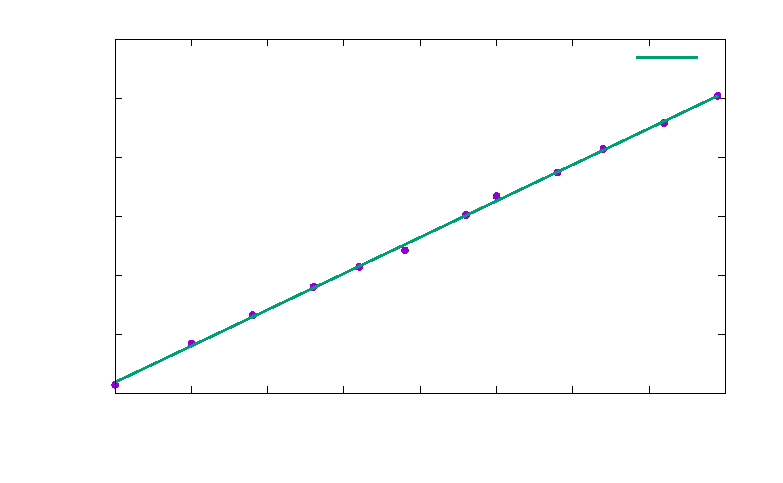
\includegraphics[width={288.00bp},height={187.20bp}]{kalibrace_proudu}}%
    \gplfronttext
  \end{picture}%
\endgroup

  \caption{závislost proudu protekájícího čidlem na výšce vodního sloupce}
\end{figure}

\subsection{Měření Clément Desormovou metodou}

Podle Clément Desormovy metody jsem postupně nepřímo měřil tlak $p_1$ před adiabatickou expanzí a tlak $p_3$ po 
izochorickém ohřevu. Výslednou Poissonovu konstantu spočítám jako sklon fitu rozdílu $p_1 - p_0$ a $p_1 - p_3$.

\begin{figure}[ht]
  \centering
  % GNUPLOT: LaTeX picture with Postscript
\begingroup
  \makeatletter
  \providecommand\color[2][]{%
    \GenericError{(gnuplot) \space\space\space\@spaces}{%
      Package color not loaded in conjunction with
      terminal option `colourtext'%
    }{See the gnuplot documentation for explanation.%
    }{Either use 'blacktext' in gnuplot or load the package
      color.sty in LaTeX.}%
    \renewcommand\color[2][]{}%
  }%
  \providecommand\includegraphics[2][]{%
    \GenericError{(gnuplot) \space\space\space\@spaces}{%
      Package graphicx or graphics not loaded%
    }{See the gnuplot documentation for explanation.%
    }{The gnuplot epslatex terminal needs graphicx.sty or graphics.sty.}%
    \renewcommand\includegraphics[2][]{}%
  }%
  \providecommand\rotatebox[2]{#2}%
  \@ifundefined{ifGPcolor}{%
    \newif\ifGPcolor
    \GPcolorfalse
  }{}%
  \@ifundefined{ifGPblacktext}{%
    \newif\ifGPblacktext
    \GPblacktexttrue
  }{}%
  % define a \g@addto@macro without @ in the name:
  \let\gplgaddtomacro\g@addto@macro
  % define empty templates for all commands taking text:
  \gdef\gplbacktext{}%
  \gdef\gplfronttext{}%
  \makeatother
  \ifGPblacktext
    % no textcolor at all
    \def\colorrgb#1{}%
    \def\colorgray#1{}%
  \else
    % gray or color?
    \ifGPcolor
      \def\colorrgb#1{\color[rgb]{#1}}%
      \def\colorgray#1{\color[gray]{#1}}%
      \expandafter\def\csname LTw\endcsname{\color{white}}%
      \expandafter\def\csname LTb\endcsname{\color{black}}%
      \expandafter\def\csname LTa\endcsname{\color{black}}%
      \expandafter\def\csname LT0\endcsname{\color[rgb]{1,0,0}}%
      \expandafter\def\csname LT1\endcsname{\color[rgb]{0,1,0}}%
      \expandafter\def\csname LT2\endcsname{\color[rgb]{0,0,1}}%
      \expandafter\def\csname LT3\endcsname{\color[rgb]{1,0,1}}%
      \expandafter\def\csname LT4\endcsname{\color[rgb]{0,1,1}}%
      \expandafter\def\csname LT5\endcsname{\color[rgb]{1,1,0}}%
      \expandafter\def\csname LT6\endcsname{\color[rgb]{0,0,0}}%
      \expandafter\def\csname LT7\endcsname{\color[rgb]{1,0.3,0}}%
      \expandafter\def\csname LT8\endcsname{\color[rgb]{0.5,0.5,0.5}}%
    \else
      % gray
      \def\colorrgb#1{\color{black}}%
      \def\colorgray#1{\color[gray]{#1}}%
      \expandafter\def\csname LTw\endcsname{\color{white}}%
      \expandafter\def\csname LTb\endcsname{\color{black}}%
      \expandafter\def\csname LTa\endcsname{\color{black}}%
      \expandafter\def\csname LT0\endcsname{\color{black}}%
      \expandafter\def\csname LT1\endcsname{\color{black}}%
      \expandafter\def\csname LT2\endcsname{\color{black}}%
      \expandafter\def\csname LT3\endcsname{\color{black}}%
      \expandafter\def\csname LT4\endcsname{\color{black}}%
      \expandafter\def\csname LT5\endcsname{\color{black}}%
      \expandafter\def\csname LT6\endcsname{\color{black}}%
      \expandafter\def\csname LT7\endcsname{\color{black}}%
      \expandafter\def\csname LT8\endcsname{\color{black}}%
    \fi
  \fi
    \setlength{\unitlength}{0.0500bp}%
    \ifx\gptboxheight\undefined%
      \newlength{\gptboxheight}%
      \newlength{\gptboxwidth}%
      \newsavebox{\gptboxtext}%
    \fi%
    \setlength{\fboxrule}{0.5pt}%
    \setlength{\fboxsep}{1pt}%
    \definecolor{tbcol}{rgb}{1,1,1}%
\begin{picture}(5760.00,3744.00)%
    \gplgaddtomacro\gplbacktext{%
      \csname LTb\endcsname%%
      \put(-75,149){\makebox(0,0)[r]{\strut{}$70$}}%
      \put(-75,505){\makebox(0,0)[r]{\strut{}$75$}}%
      \put(-75,860){\makebox(0,0)[r]{\strut{}$80$}}%
      \put(-75,1216){\makebox(0,0)[r]{\strut{}$85$}}%
      \put(-75,1571){\makebox(0,0)[r]{\strut{}$90$}}%
      \put(-75,1927){\makebox(0,0)[r]{\strut{}$95$}}%
      \put(-75,2283){\makebox(0,0)[r]{\strut{}$100$}}%
      \put(-75,2638){\makebox(0,0)[r]{\strut{}$105$}}%
      \put(-75,2994){\makebox(0,0)[r]{\strut{}$110$}}%
      \put(-75,3349){\makebox(0,0)[r]{\strut{}$115$}}%
      \put(-75,3705){\makebox(0,0)[r]{\strut{}$120$}}%
      \put(57,-71){\makebox(0,0){\strut{}$55$}}%
      \put(863,-71){\makebox(0,0){\strut{}$60$}}%
      \put(1670,-71){\makebox(0,0){\strut{}$65$}}%
      \put(2476,-71){\makebox(0,0){\strut{}$70$}}%
      \put(3282,-71){\makebox(0,0){\strut{}$75$}}%
      \put(4088,-71){\makebox(0,0){\strut{}$80$}}%
      \put(4895,-71){\makebox(0,0){\strut{}$85$}}%
      \put(5701,-71){\makebox(0,0){\strut{}$90$}}%
    }%
    \gplgaddtomacro\gplfronttext{%
      \csname LTb\endcsname%%
      \put(-680,1927){\rotatebox{-270.00}{\makebox(0,0){\strut{}$h_1$ [mm]}}}%
      \put(2879,-401){\makebox(0,0){\strut{}$h_1$ - $h_3$ [mm]}}%
    }%
    \gplbacktext
    \put(0,0){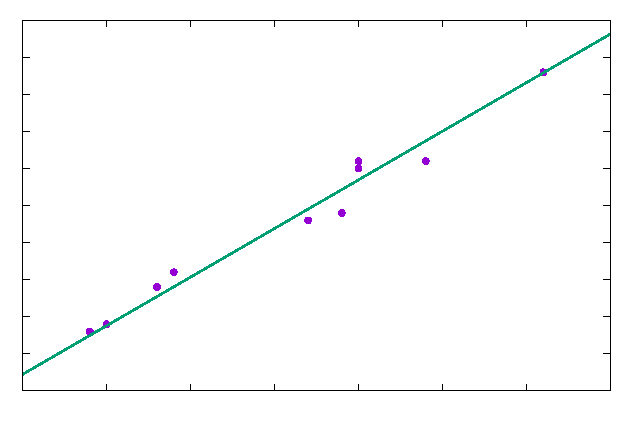
\includegraphics[width={288.00bp},height={187.20bp}]{clement}}%
    \gplfronttext
  \end{picture}%
\endgroup

  \caption{závislost rozdílu naměřených hodnot $h_1 - h_3$, na $h_1$}
\end{figure}

\newpage

\begin{figure}[ht]
  \centering
  % GNUPLOT: LaTeX picture with Postscript
\begingroup
  \makeatletter
  \providecommand\color[2][]{%
    \GenericError{(gnuplot) \space\space\space\@spaces}{%
      Package color not loaded in conjunction with
      terminal option `colourtext'%
    }{See the gnuplot documentation for explanation.%
    }{Either use 'blacktext' in gnuplot or load the package
      color.sty in LaTeX.}%
    \renewcommand\color[2][]{}%
  }%
  \providecommand\includegraphics[2][]{%
    \GenericError{(gnuplot) \space\space\space\@spaces}{%
      Package graphicx or graphics not loaded%
    }{See the gnuplot documentation for explanation.%
    }{The gnuplot epslatex terminal needs graphicx.sty or graphics.sty.}%
    \renewcommand\includegraphics[2][]{}%
  }%
  \providecommand\rotatebox[2]{#2}%
  \@ifundefined{ifGPcolor}{%
    \newif\ifGPcolor
    \GPcolorfalse
  }{}%
  \@ifundefined{ifGPblacktext}{%
    \newif\ifGPblacktext
    \GPblacktexttrue
  }{}%
  % define a \g@addto@macro without @ in the name:
  \let\gplgaddtomacro\g@addto@macro
  % define empty templates for all commands taking text:
  \gdef\gplbacktext{}%
  \gdef\gplfronttext{}%
  \makeatother
  \ifGPblacktext
    % no textcolor at all
    \def\colorrgb#1{}%
    \def\colorgray#1{}%
  \else
    % gray or color?
    \ifGPcolor
      \def\colorrgb#1{\color[rgb]{#1}}%
      \def\colorgray#1{\color[gray]{#1}}%
      \expandafter\def\csname LTw\endcsname{\color{white}}%
      \expandafter\def\csname LTb\endcsname{\color{black}}%
      \expandafter\def\csname LTa\endcsname{\color{black}}%
      \expandafter\def\csname LT0\endcsname{\color[rgb]{1,0,0}}%
      \expandafter\def\csname LT1\endcsname{\color[rgb]{0,1,0}}%
      \expandafter\def\csname LT2\endcsname{\color[rgb]{0,0,1}}%
      \expandafter\def\csname LT3\endcsname{\color[rgb]{1,0,1}}%
      \expandafter\def\csname LT4\endcsname{\color[rgb]{0,1,1}}%
      \expandafter\def\csname LT5\endcsname{\color[rgb]{1,1,0}}%
      \expandafter\def\csname LT6\endcsname{\color[rgb]{0,0,0}}%
      \expandafter\def\csname LT7\endcsname{\color[rgb]{1,0.3,0}}%
      \expandafter\def\csname LT8\endcsname{\color[rgb]{0.5,0.5,0.5}}%
    \else
      % gray
      \def\colorrgb#1{\color{black}}%
      \def\colorgray#1{\color[gray]{#1}}%
      \expandafter\def\csname LTw\endcsname{\color{white}}%
      \expandafter\def\csname LTb\endcsname{\color{black}}%
      \expandafter\def\csname LTa\endcsname{\color{black}}%
      \expandafter\def\csname LT0\endcsname{\color{black}}%
      \expandafter\def\csname LT1\endcsname{\color{black}}%
      \expandafter\def\csname LT2\endcsname{\color{black}}%
      \expandafter\def\csname LT3\endcsname{\color{black}}%
      \expandafter\def\csname LT4\endcsname{\color{black}}%
      \expandafter\def\csname LT5\endcsname{\color{black}}%
      \expandafter\def\csname LT6\endcsname{\color{black}}%
      \expandafter\def\csname LT7\endcsname{\color{black}}%
      \expandafter\def\csname LT8\endcsname{\color{black}}%
    \fi
  \fi
    \setlength{\unitlength}{0.0500bp}%
    \ifx\gptboxheight\undefined%
      \newlength{\gptboxheight}%
      \newlength{\gptboxwidth}%
      \newsavebox{\gptboxtext}%
    \fi%
    \setlength{\fboxrule}{0.5pt}%
    \setlength{\fboxsep}{1pt}%
    \definecolor{tbcol}{rgb}{1,1,1}%
\begin{picture}(5760.00,3744.00)%
    \gplgaddtomacro\gplbacktext{%
      \csname LTb\endcsname%%
      \put(-75,149){\makebox(0,0)[r]{\strut{}$2$}}%
      \put(-75,505){\makebox(0,0)[r]{\strut{}$2.2$}}%
      \put(-75,860){\makebox(0,0)[r]{\strut{}$2.4$}}%
      \put(-75,1216){\makebox(0,0)[r]{\strut{}$2.6$}}%
      \put(-75,1571){\makebox(0,0)[r]{\strut{}$2.8$}}%
      \put(-75,1927){\makebox(0,0)[r]{\strut{}$3$}}%
      \put(-75,2283){\makebox(0,0)[r]{\strut{}$3.2$}}%
      \put(-75,2638){\makebox(0,0)[r]{\strut{}$3.4$}}%
      \put(-75,2994){\makebox(0,0)[r]{\strut{}$3.6$}}%
      \put(-75,3349){\makebox(0,0)[r]{\strut{}$3.8$}}%
      \put(-75,3705){\makebox(0,0)[r]{\strut{}$4$}}%
      \put(57,-71){\makebox(0,0){\strut{}$1.6$}}%
      \put(925,-71){\makebox(0,0){\strut{}$1.8$}}%
      \put(1794,-71){\makebox(0,0){\strut{}$2$}}%
      \put(2662,-71){\makebox(0,0){\strut{}$2.2$}}%
      \put(3530,-71){\makebox(0,0){\strut{}$2.4$}}%
      \put(4399,-71){\makebox(0,0){\strut{}$2.6$}}%
      \put(5267,-71){\makebox(0,0){\strut{}$2.8$}}%
    }%
    \gplgaddtomacro\gplfronttext{%
      \csname LTb\endcsname%%
      \put(-680,1927){\rotatebox{-270.00}{\makebox(0,0){\strut{}$I_1$ - $I_0$ [mA]}}}%
      \put(2879,-401){\makebox(0,0){\strut{}$I_1$ - $I_3$ [mA]}}%
    }%
    \gplbacktext
    \put(0,0){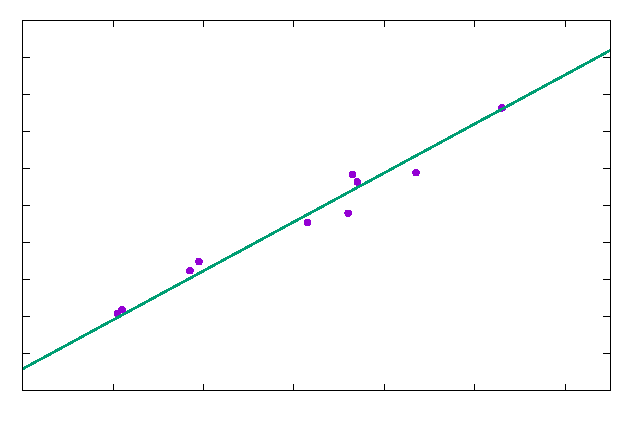
\includegraphics[width={288.00bp},height={187.20bp}]{clement-cidlem}}%
    \gplfronttext
  \end{picture}%
\endgroup

  \caption{závislost rozdílu naměřených hodnot $I_1 - I_3$, na $I_1 - I_0$}
\end{figure}

\begin{table}[ht]
  \centering
  \begin{tabular}{c | c }
    metoda & $\kappa$ \\ \hline\hline
    pomocí U trubice & $(1.31 \pm 0.04)$ \\
    pomocí kalibrace & $(1.32 \pm 0.04)$ \\ \hline
  \end{tabular}
  \caption{Hodnoty spočítané z grafu 2 a 3 Použitím vztahu (8)}
\end{table}

\subsection{Kundutovou trubicí}

V Kundutově trubici je posuvka nastavující její délku, generátor sinusového signálu a osciloskop. Na osciloskopu nastavím vhodnou frekvenci a posuvkou postupně prodlužuji její délku. Rozdíl každých dvou amplitud vzniklého interferenčního vlnění měřené osciloskopem odpovídá půlce vlnové délky. Výsledky pro 4 různé frekvence jsou uvedené v tabulce 2.

\begin{figure}[htpb]
  \centering
  % GNUPLOT: LaTeX picture with Postscript
\begingroup
  \makeatletter
  \providecommand\color[2][]{%
    \GenericError{(gnuplot) \space\space\space\@spaces}{%
      Package color not loaded in conjunction with
      terminal option `colourtext'%
    }{See the gnuplot documentation for explanation.%
    }{Either use 'blacktext' in gnuplot or load the package
      color.sty in LaTeX.}%
    \renewcommand\color[2][]{}%
  }%
  \providecommand\includegraphics[2][]{%
    \GenericError{(gnuplot) \space\space\space\@spaces}{%
      Package graphicx or graphics not loaded%
    }{See the gnuplot documentation for explanation.%
    }{The gnuplot epslatex terminal needs graphicx.sty or graphics.sty.}%
    \renewcommand\includegraphics[2][]{}%
  }%
  \providecommand\rotatebox[2]{#2}%
  \@ifundefined{ifGPcolor}{%
    \newif\ifGPcolor
    \GPcolorfalse
  }{}%
  \@ifundefined{ifGPblacktext}{%
    \newif\ifGPblacktext
    \GPblacktexttrue
  }{}%
  % define a \g@addto@macro without @ in the name:
  \let\gplgaddtomacro\g@addto@macro
  % define empty templates for all commands taking text:
  \gdef\gplbacktext{}%
  \gdef\gplfronttext{}%
  \makeatother
  \ifGPblacktext
    % no textcolor at all
    \def\colorrgb#1{}%
    \def\colorgray#1{}%
  \else
    % gray or color?
    \ifGPcolor
      \def\colorrgb#1{\color[rgb]{#1}}%
      \def\colorgray#1{\color[gray]{#1}}%
      \expandafter\def\csname LTw\endcsname{\color{white}}%
      \expandafter\def\csname LTb\endcsname{\color{black}}%
      \expandafter\def\csname LTa\endcsname{\color{black}}%
      \expandafter\def\csname LT0\endcsname{\color[rgb]{1,0,0}}%
      \expandafter\def\csname LT1\endcsname{\color[rgb]{0,1,0}}%
      \expandafter\def\csname LT2\endcsname{\color[rgb]{0,0,1}}%
      \expandafter\def\csname LT3\endcsname{\color[rgb]{1,0,1}}%
      \expandafter\def\csname LT4\endcsname{\color[rgb]{0,1,1}}%
      \expandafter\def\csname LT5\endcsname{\color[rgb]{1,1,0}}%
      \expandafter\def\csname LT6\endcsname{\color[rgb]{0,0,0}}%
      \expandafter\def\csname LT7\endcsname{\color[rgb]{1,0.3,0}}%
      \expandafter\def\csname LT8\endcsname{\color[rgb]{0.5,0.5,0.5}}%
    \else
      % gray
      \def\colorrgb#1{\color{black}}%
      \def\colorgray#1{\color[gray]{#1}}%
      \expandafter\def\csname LTw\endcsname{\color{white}}%
      \expandafter\def\csname LTb\endcsname{\color{black}}%
      \expandafter\def\csname LTa\endcsname{\color{black}}%
      \expandafter\def\csname LT0\endcsname{\color{black}}%
      \expandafter\def\csname LT1\endcsname{\color{black}}%
      \expandafter\def\csname LT2\endcsname{\color{black}}%
      \expandafter\def\csname LT3\endcsname{\color{black}}%
      \expandafter\def\csname LT4\endcsname{\color{black}}%
      \expandafter\def\csname LT5\endcsname{\color{black}}%
      \expandafter\def\csname LT6\endcsname{\color{black}}%
      \expandafter\def\csname LT7\endcsname{\color{black}}%
      \expandafter\def\csname LT8\endcsname{\color{black}}%
    \fi
  \fi
    \setlength{\unitlength}{0.0500bp}%
    \ifx\gptboxheight\undefined%
      \newlength{\gptboxheight}%
      \newlength{\gptboxwidth}%
      \newsavebox{\gptboxtext}%
    \fi%
    \setlength{\fboxrule}{0.5pt}%
    \setlength{\fboxsep}{1pt}%
    \definecolor{tbcol}{rgb}{1,1,1}%
\begin{picture}(7200.00,3456.00)%
    \gplgaddtomacro\gplbacktext{%
      \csname LTb\endcsname%%
      \put(-60,138){\makebox(0,0)[r]{\strut{}$0$}}%
      \put(-60,607){\makebox(0,0)[r]{\strut{}$20$}}%
      \put(-60,1076){\makebox(0,0)[r]{\strut{}$40$}}%
      \put(-60,1545){\makebox(0,0)[r]{\strut{}$60$}}%
      \put(-60,2013){\makebox(0,0)[r]{\strut{}$80$}}%
      \put(-60,2482){\makebox(0,0)[r]{\strut{}$100$}}%
      \put(-60,2951){\makebox(0,0)[r]{\strut{}$120$}}%
      \put(-60,3420){\makebox(0,0)[r]{\strut{}$140$}}%
      \put(72,-82){\makebox(0,0){\strut{}$0$}}%
      \put(1483,-82){\makebox(0,0){\strut{}$5$}}%
      \put(2894,-82){\makebox(0,0){\strut{}$10$}}%
      \put(4305,-82){\makebox(0,0){\strut{}$15$}}%
      \put(5716,-82){\makebox(0,0){\strut{}$20$}}%
      \put(7127,-82){\makebox(0,0){\strut{}$25$}}%
    }%
    \gplgaddtomacro\gplfronttext{%
      \csname LTb\endcsname%%
      \put(6140,3247){\makebox(0,0)[r]{\strut{}f = 1.56 kHz}}%
      \csname LTb\endcsname%%
      \put(6140,3027){\makebox(0,0)[r]{\strut{}f = 1.89 kHz}}%
      \csname LTb\endcsname%%
      \put(6140,2807){\makebox(0,0)[r]{\strut{}f = 3.41 kHz}}%
      \csname LTb\endcsname%%
      \put(6140,2587){\makebox(0,0)[r]{\strut{}f = 5.04 kHz}}%
      \csname LTb\endcsname%%
      \put(-665,1779){\rotatebox{-270.00}{\makebox(0,0){\strut{}l [cm]}}}%
      \put(3599,-412){\makebox(0,0){\strut{}n-té měření}}%
    }%
    \gplbacktext
    \put(0,0){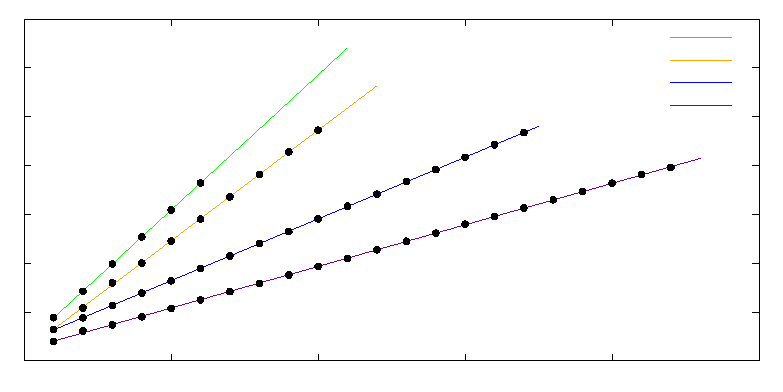
\includegraphics[width={360.00bp},height={172.80bp}]{vlnova_delka}}%
    \gplfronttext
  \end{picture}%
\endgroup

  \caption{závislost n-tého maxima amplitudy vlnění na vzdálenosti}
\end{figure}

\begin{table}[ht]
  \centering
  \begin{tabular}{| c | c | c | c |}
    \hline
    $f$ [kHz] & $\frac{\lambda }{2}$ [cm] & v$_\text{vzduchu}$ [ms$^{-1}$] & $\kappa$ \\ \hline
    1.56 & $11.06 \pm 0.02$  & $345.1 \pm 0.4$ & $1.4 \pm 0.2$ \\
    1.89 & $9.06  \pm 0.04$  & $342.5 \pm 0.8$ & $1.4 \pm 0.3 $\\
    3.41 & $5.05 \pm 0.004$  & $344.41 \pm 0.08$ & $1.40 \pm 0.03$ \\
    5.04 & $3.403 \pm 0.008$ & $343.02 \pm 0.02$ & $1.39 \pm 0.03$ \\ \hline
  \end{tabular}
  \caption{Hodnoty spočítané z grafu 2}
\end{table}

\section{Závěr}

Opravdová poissonova konstanta pro vzduch za laboratorních podmínek $\kappa \approx 1.40.$ \\

 Měření Clément Desormovou metodou je chybné asi o 7 \%. Myslím, že jsem pokaždé zavřel ventil na nádobě moc brzo a tlaky se nestihli vyrovnat.
Proto je naměřená hodnota menší než skutečná. Měření Kundutovou trubicí je na druhou stranu docela přesné. 
Je i vidět, že pro větší hodnoty frekvence klesá vlnová délka, což zjednodušuje hledání maxima a vede k přesnějšímu měření.


\begin{thebibliography}{0}
\bibitem{hustota vzduchu} kalkulačka hustoty vzduchu \url{https://www.omnicalculator.com/physics/air-density}.
\end{thebibliography}

\end{document}

